

In this chapter we give an overview of \maestroex, including some of the
standard problems, how to run the code, some basic runtime parameters,
and how to look at the output.

%-----------------------------------------------------------------------------
% Quick Start
%-----------------------------------------------------------------------------
\section{Quick Start}

Here we will run the standard {\tt reacting\_bubble} problem (three
reacting bubbles in a plane-parallel stratified atmosphere) on a
single processor\footnote{In earlier versions of \maestroex\ this
problem was called {\tt test2}}.  This test problem was shown in
paper~3.

\begin{enumerate}

\item {\em Get a copy of \maestroex}.

  If you don't already have a copy of \maestroex, you can obtain one
  from the project's {\sf github} page:
  \url{https://github.com/AMReX-Astro/MAESTROeX}\, .  There are several
  options: you can fork it directly on {\sf github} (recommended if
  you intend to develop the code) or clone it using {\tt git} from the
  project page.

  \maestroex\ is under active development, so you will want to keep in
  sync with the changes by periodically pulling from the repository.
  Simply type
  \begin{verbatim}
git pull
  \end{verbatim}
  in the {\tt MAESTROeX/} directory.

\item {\em Get a copy of \microphysics}.

  \maestroex\ and its compressible counterpart \castro\ share a
  common-set of microphysics solvers (nuclear reaction networks and
  equations of state).  These are kept in a separate repo.
  \microphysics\ is also available on github and can be obtained 
  via:
  \begin{verbatim}
git clone https://github.com/starkiller-astro/Microphysics.git
  \end{verbatim}

  You will periodic want to update \microphysics\ by doing
  \begin{verbatim}
git pull
  \end{verbatim}
  in the {\tt Microphysics/} directory
.
\item {\em Get a copy of \amrex}.

  \maestroex\ requires the \amrex\ library to manage the grids and
  parallelization.  We also rely on the build system in \amrex\ to
  build a \maestroex\ executable.  \amrex\ is also available on github
  and can be obtained via:
  \begin{verbatim}
git clone https://github.com/AMReX-Codes/amrex.git
  \end{verbatim}

  You will periodic want to update \amrex\ by doing
  \begin{verbatim}
git pull
  \end{verbatim}
  in the {\tt amrex/} directory.


\item {\em Setup your shell environment}.

  \maestroex\ needs to know where to find \amrex, by specifying the
  {\tt AMREX\_HOME} environment variable, and where
  to find \microphysics, bt specifying the {\tt
  MICROPHYSICS\_HOME} environment variable.

  If your shell is {\tt Bash}, add
  \begin{verbatim}
export AMREX_HOME="/path/to/amrex/"
export MICROPHYSICS_HOME="/path/to/Microphysics/"
  \end{verbatim}
  to your {\tt .bashrc}. 

  If your shell is {\tt Csh/Tcsh}, add
  \begin{verbatim}
setenv AMREX_HOME /path/to/amrex/
setenv MICROPHYSICS_HOME /path/to/Microphysics/
  \end{verbatim}
  to your {\tt .cshrc}.  

  Note: you must specify the full path to the {\tt AMReX/} and {\tt
    Microphysics/} directory.  Do not use ``$\sim$'' to refer to your
  home directory---the scripts used by the build system will not be
  able to process this.

\item {\em Setup the problem's {\tt GNUmakefile}}.

  In \maestroex, each problem lives under one of three sub-directories
  of {\tt MAESTROeX/Exec}: {\tt SCIENCE/}, {\tt TEST\_PROBLEMS/}, or
  {\tt UNIT\_TESTS/}.  This problem sub-directory will contain any
  problem-specific files as well as the {\tt GNUmakefile} that
  specifies how to build the executable.  Note: we rely on features of
  GNU {\tt make}.  Full details of the {\tt GNUmakefile} can be found
  in \S~\ref{sec:adding_problems}.  Here we will configure for a
  serial build.

  Change directory to 
  {\tt MAESTROeX/Exec/TEST\_PROBLEMS/reacting\_bubble/}.
  We only need to worry about the options at the very top of the 
  {\tt GNUmakefile} for now.  These should be set as follows:
  \begin{itemize}

  \item {\tt DEBUG := TRUE}

    This option determines whether we compile with support for 
    less-optimized code with debugging runtime checks.  Setting 
    {\tt DEBUG := FALSE} turns off debugging.

  \item {\tt DIM := 2}

    The dimensionality of the problem must be specified at compile-time.

  \item {\tt COMP := gnu}

    This option specifies the gnu compiler suite (g++/gfortran).  
    We will use {\tt gnu}, which is the preferred compiler suite for \maestroex.
    Specifying this compiler will automatically pull in the compiler
    settings as specified in {\tt AMREX\_HOME/Tools/GNUMake/Make.defs}.
    (Alternate compiler choices include 
    {\tt intel}, {\tt cray}, and {\tt pgi}.

  \item {\tt USE\_MPI := TRUE}

    This determines whether we are doing a parallel build, using the
    Message Passing Interface (MPI) library.  If you set this option
    to {\tt FALSE}, you will disable MPI
    and will build \maestroex\ in serial
    mode, so no MPI library needs to be present on the host system.

  \item {\tt USE\_OMP := FALSE}

    This determines whether we are using OpenMP to do parallelism
    within a shared memory node.  OpenMP is used together with MPI,
    with MPI distributing the grids across the processors and within a
    shared-memory node, OpenMP allows many cores to operate on the
    same grid.  For now, we leave this option as {\tt FALSE}, disabling OpenMP.

  \item {\tt USE\_REACT := TRUE}

    Some test problems in \maestroex\ do not use reactions, so there is an
    option to disable the compilation of reaction-specific source code.

  \item {\tt TINY\_PROFILE := FALSE}

    Profiling tool that generates a text file with profiling information.
    Refer to the \amrex\ User's Guide at 
    \url{https://amrex-codes.github.io/amrex/}

  \item {\tt PROFILE := FALSE}

    More advanced profiling tool that generates a text file with profiling 
    information, or data files that can be interpreted with a special build of 
    {\tt amrvis}.  Selecting {\tt TRUE} overrides the {\tt TINY\_PROFILE} setting.
    Refer to the \amrex\ User's Guide at \url{https://amrex-codes.github.io/amrex/}

  \end{itemize}


\item {\em Build the executable}.

  Type {\tt make}.  The build system will first find the dependencies
  amongst all the source files and then build the executable.  When
  finished, the executable will have a name like
  {\tt Maestro2d.gnu.DEBUG.MPI.ex}, where the specific parts of the name
  depend on the options used in {\tt GNUmakefile}.

  Note, at the end of the build process, a link will be made in the
  current directory to the data table needed for the equation of state
  ({\tt Microphysics/EOS/helmholtz/helm\_table.dat}).


\item {\em Run!}

  Each problem requires an input file.  The inputs file
  consists of lines of the form {\em parameter = value},
  where {\em parameter} is one of the many runtime parameters
  \maestroex\ knows, and {\em value} overrides the default value for
  that parameter.  For the {\tt reacting\_bubble} problem, we will use
  the inputs file {\tt inputs\_2d\_C}.  An overview of some of the more
  common runtime parameters is given in
  \S~\ref{sec:gettingstarted:runtime}, and a full list of all
  \maestroex\ runtime parameters and their default values is given in
  Chapter~\ref{ch:runtimeparameters}.

  \maestroex\ is run simply as:
  \begin{verbatim}
  ./Maestro2d.gnu.DEBUG.MPI.ex inputs_2d_C
  \end{verbatim}
  or to run in parallel on a local workstation:
  \begin{verbatim}
  mpiexec -n 4 ./Maestro2d.gnu.DEBUG.MPI.ex inputs_2d_C
  \end{verbatim}
  We can also override the default value of any runtime parameter by
  specifying it on the commandline as, e.g.,
  \begin{verbatim}
  ./Maestro2d.gnu.DEBUG.MPI.ex inputs_2d_C maestro.max_step=0 amr.n_cell=192 320
  \end{verbatim}

  As the code runs, a lot of information will pass through the screen.
  For each timestep, each of the steps 1 through 12 shown in the
  \maestroex\ flowchart (Chapter~\ref{ch:flowchart}) will be shown along
  with diagnostic information about the solution.  Upon completion
  some memory usage information is printed.


\item {\em Examine the output}.
  
  As the code runs, it will output both plotfiles and checkpoints as
  well as one or more text diagnostic files ({\tt maestro\_diag.out}
  by default) with integral or extrema information (like maximum Mach
  number) from each timestep.

  By default, the plotfiles will be named {\tt plt}{\em nnnnnnn}, where
  the number {\em nnnnnnn} is the timestep number when the file was
  outputted.  Similarly, the checkpoints are named
  {\tt chk}{\em nnnnnnn}.  \amrex\ plotfiles and checkpoints are actually
  directories, with the data stored in sub-directories grouped by
  refinement level.  Details of the simulation (build information,
  number of processors used, output date, output directory, runtime
  parameter values, ...)  are stored in the plaintext {\tt job\_info}
  file in each plotfile and checkpoint directory.

  {\bf Note: unless otherwise specified all quantities in
    \maestroex\ are assumed to be in CGS units.}

  Visualization of results is described in the next section.


\end{enumerate}


\section{Working with the Output}

Visualization and analysis are done on the plotfiles.  A number of
in-house and externally developed tools can work with \amrex-formatted
plotfiles\footnote{The plotfiles are in the same format as those made
  by the \boxlib\ library upon which \maestroex\ was previously based.}.
An example plot of the {\tt reacting\_bubble} problem run above is
shown in Figure~\ref{fig:gettingstarted:test2}.

\begin{figure}[t]
\centering
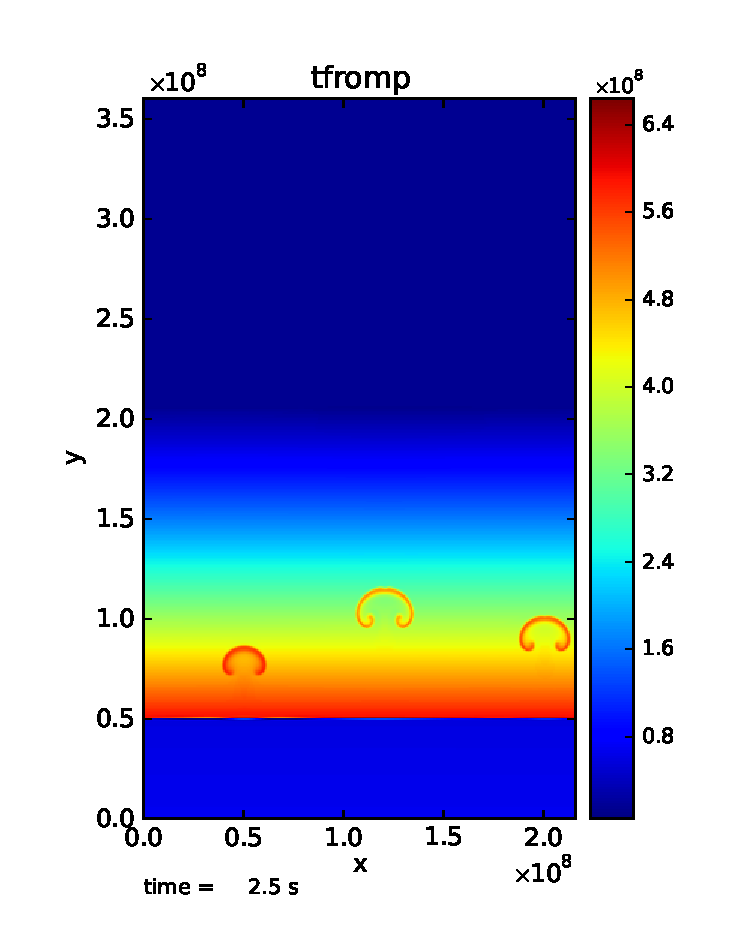
\includegraphics[width=3in]{\gsfigpath/plt00133_tfromp}
\caption[Visualization of {\tt reacting\_bubble} output]{\label{fig:gettingstarted:test2} Visualization of the
final output of the {\tt reacting\_bubble} problem showing the temperature
field (as derived from the pressure).  This plot was done with
the {\tt AmrPostprocessing} tools.}
\end{figure}



\subsection{\amrvis}

\amrvis\ is an easy-to-use visualization tool developed at LBL for
2- and 3D datasets which can plot slices through 3D datasets as well
as volume-renderings.  It can also very easily extract 1D lines
through the dataset along any coordinate direction.  It is distributed
separately from the \maestroex\ distribution.

\amrvis\ can be obtained via git from github as:
\begin{verbatim}
git clone https://github.com/AMReX-Codes/Amrvis.git
\end{verbatim}
Also, to build a 3D version of \amrvis\ you need to obtain volpack using:
\begin{verbatim}
git clone https://ccse.lbl.gov/pub/Downloads/volpack.git
\end{verbatim}
\amrvis\ is built in the C++ \amrex\ framework (instead of the Fortran 
\amrex\ framework that \maestroex\ uses).  The build systems are similar,
but differ in a few ways.  

\amrvis\ uses the {\tt Motif} library for defining the GUI.  On a Linux 
system, you may need to install the {\tt lesstif} package and any
related development packages (e.g.\ {\tt lesstif-devel}).  Depending
on your Linux system, you may also need to install {\tt libXpm} and
related development packages (e.g.\ {\tt libXpm-devel}).  

Further details on the C++ \amrex\ build system used by \amrvis\
can be found in the \amrex\ documentation.

\subsection{{\tt AmrPostprocessing} scripts}

Several useful analysis scripts (written in Fortran 90) can be found
in {\tt amrex/Tools/Postprocessing/F\_Src/}.
The {\tt GNUmakefile} there needs to be edited to
indicate which of the tools to build.  For example, to extract the
density along a line from the center of a plotfile, {\tt plt00200}, in
the $y$-direction:

\begin{verbatim}
fextract.Linux.gfortran.exe -d 2 -v "density" -p plt00200
\end{verbatim}

These routines are described in \S~\ref{sec:analysis}.

There is also a python visualization method in {\tt
AmrPostprocessing/python}.  This is described
in \S~\ref{sec:vis:python}.


\subsection{\visit}

\visit\ is a powerful, DOE-supported visualization tool for 2- and 3D
datasets.  It can do contouring, volume rendering, streamlines, ...\, ,
directly from \amrex\ plotfiles.   Details on
\visit\ can be found at:\newline
 \url{https://wci.llnl.gov/codes/visit/home.html}\,. \newline
The easiest way to get started with \visit\ is to download a precompiled
binary from the \visit\ webpage.

Once \visit\ is installed, you can open a \amrex\ plotfile by pointing
\visit\ to the {\tt Header} file in the plotfile directory.


\subsection{\yt}

\yt\ (version 3.0 and later) can natively read the \maestroex\ plotfiles.  See
the \yt\ documentation or \S~\ref{sec:vis:yt}.



\subsection{Diagnostic Files}

By default, \maestroex\ outputs global diagnostics each timestep into a
file called {\tt maestro\_diag.out}.  This includes the maximum Mach
number, peak temperature, and peak nuclear energy generation rate.
Individual problems can provide their own \code{diag.f90} file to
produce custom diagnostic output.  This information can be plotted
directly with {\sf GNUplot}, for example.




\section{`Standard' Test Problems}

Different problems in \maestroex\ are contained in one of three
sub-directories under {\tt MAESTROeX/Exec}: ({\tt SCIENCE/}, {\tt
TEST\_PROBLEMS/}, or {\tt UNIT\_TESTS/}).  The {\tt GNUmakefile} in each
problem directory lists the components of {\tt MAESTRO} that are used
to build the executable.  {\tt TEST\_PROBLEMS/} contains simple
problems that were used in the development of \maestroex.  Many
of these were featured in the papers describing the \maestroex\ algorithm.

Some of the test problems available are:
\begin{itemize}
\item {\tt double\_bubble} \\[-3mm]

A rising bubble problem where the bubble(s) can have a different gamma
than the surrounding atmosphere.  This uses the {\tt multigamma} EOS.

\item {\tt incomp\_shear\_jet} \\[-3mm]

A simple pure-incompressible shear layer problem.  This is the example
problem used in \cite{bellcolellaglaz}.  This is useful to see how to
use \maestroex\ as an incompressible solver.

\item {\tt reacting\_bubble} \\[-3mm]

{\tt reacting\_bubble} places 3 hots spots in a plane-parallel atmosphere.
Burning makes these bubbles buoyant, and then roll up.  This problem was
used in \cite{lowMach3} to compare with compressible solvers.

This problem can also be run adaptively.  The \code{tag\_boxes.f90}
file in the problem directory tags cells for refinement if the
perturbational temperature, $T^\prime$, exceeds some threshold.  

\item {\tt rt} \\ [-3mm]

A Rayleigh-Taylor instability problem.  There are two methods that the
code is run here, in the standard (using {\tt inputs\_2d}), the base state
has the stratified atmosphere and we introduce a velocity perturbation
to start the instability.  The alternate method, {\tt inputs\_2d\_SNe}, uses
the \runparam{do\_smallscale} runtime parameter to eliminate the base state
and instead use the incompressible constraint to evolve the system.

\item {\tt test\_convect} \\[-3mm]

{\tt test\_convect} drives convection through a plane-parallel
atmosphere using an externally-specified heat source.  This problem
was used to compare with compressible solvers in \cite{lowMach3}
and to test the multilevel algorithm in \cite{multilevel}.

\item {\tt test\_spherical} \\[-3mm]

This problem sets up an isentropically stratified star and stirs it up
with a random velocity field.  The low Mach number constraint is
replaced with the anelastic constraint (through
the \runparam{beta\_type} runtime parameter).  Analytically, under
these conditions, the density of the star should not change.  This
test problem was discussed in Maestro paper IV~\cite{lowMach4}.


\end{itemize}


\section{Distributed Science Problems}

The following problems were used for science studies.  It is
anticipated that more will be made available with time.

\begin{itemize}

\item {\tt flame} \\[-3mm]

   A combustion-mode problem where we model a thermonuclear flame in a
   small domain.  This enforces the low Mach combustion constraint
   div{U} = S.  Hot ash and cool fuel are put into contact and a flame
   will ignite and propagate across the grid.  Inflow boundary
   conditions are used to allow for an inflow velocity to be set to
   keep the laminar flame stationary.

   In this mode, \maestroex\ behaves like the code described
   in \cite{SNe}, which was used for models of Rayleigh-Taylor
   unstable flames~\cite{SNld,SNrt,SNrt3d}.

\item {\tt flame\_1d} \\[-3mm]

   A 1-d version of the {\tt flame} problem above.  This uses a special
   elliptic solver in \amrex\ that only works for a single grid, so
   no parallel runs are allowed for this problem.
   
\item {\tt toy\_convect} \\[-3mm]

A nova-like problem for studying convection.  This problem has seen
extensive use in understanding which prediction types are the best
when we have sharp species gradients.  See Mike Z or Ryan for details.

\item {\tt wdconvect} \\[-3mm]

Model convection leading up to ignition in the Chandraseskhar-mass SNe
Ia progenitor model.  This setup was the basis for the simulations
presented in \cite{lowMach4,wdconvect,wdturb}.


\end{itemize}


\section{Common Runtime Parameters}
\label{sec:gettingstarted:runtime}

\subsection{Controlling Timestepping and Output}

Parameters that set the maximum time for the simulation to run
include:
\begin{itemize}
\item \runparam{stop\_time} is the maximum simulation time, in seconds,
      to evolve the system for.

\item \runparam{max\_step} is the maximum number of steps to take.
\end{itemize}

\noindent Parameters affecting the size of the timestep include:
\begin{itemize}
\item \runparam{cflfac} is a multiplicative factor ({\tt $\le 1$}) 
      applied to the advective CFL timestep

\item \runparam{init\_shrink} is the factor ({\tt $\le 1$}) by which to reduce 
      the initial timestep from the estimated first timestep.
\end{itemize}

\noindent Parameters affecting output and restart include:
\begin{itemize}

\item \runparam{restart} tells \maestroex\ to restart from a checkpoint.  The
      value of this parameter should be the file number to restart from.
      For example, to restart from the checkpoint file {\tt chk00010},
      you would set {\tt restart = 10}.

\item \runparam{plot\_int} is the number of steps to take between
  outputting a plotfile

\item \runparam{plot\_deltat} is the simulation time to evolve between
  outputting a plotfile.  Note: to output only based on simulation
  time, set {\tt plot\_int = -1}.

\item \runparam{check\_int} is the number of steps to take between
  outputting a checkpoint.

\item \runparam{plot\_base\_name} is the basename to use for the
  plotfile filename.  The step number will be appended to
  this name.

\end{itemize}

Note that in addition to the normal plotfiles, there are {\em mini} plotfiles
that store a small subset of the fields, intended to be output more frequently.
These are described in \S~\ref{vis:sec:miniplotfile}.

\subsection{Defining the Grid and Boundary Conditions}

Parameters that determine the spatial extent of the grid, 
the types of boundaries, and the number of computational cells include:
\begin{itemize}

\item \runparam{max\_levs} is the maximum number of grid levels in the AMR
  hierarchy to use.  {\tt max\_levs = 1} indicates running with only a
  single level spanning the whole domain.

\item \runparam{n\_cellx}, \runparam{n\_celly}, \runparam{n\_cellz} the size of
  base level in terms of number of cells, in the $x$, $y$, and $z$
  coordinate directions.

\item \runparam{max\_grid\_size} the maximum extend of a grid, in any
  coordinate direction, as measured in terms of number of cells.

  For multilevel problems, the parameter \runparam{max\_grid\_size\_1}
  controls the maximum extent on level 1 (the base
  grid), \runparam{max\_grid\_size\_2} controls the maximum extent on
  level 2, and \runparam{max\_grid\_size\_3} controls the maximum extent on
  levels 3 and higher.

\item \runparam{prob\_lo\_x}, \runparam{prob\_lo\_y}, \runparam{prob\_lo\_z} is
  the physical coordinate of the lower extent of the domain boundary
  in the $x$, $y$, and $z$ coordinate directions.

\item \runparam{prob\_hi\_x}, \runparam{prob\_hi\_y}, \runparam{prob\_hi\_z} is
  the physical coordinate of the upper extent of the domain boundary
  in the $x$, $y$, and $z$ coordinate directions.

\item There are two ways to specify boundary conditions---via integer flags
      or descriptive string names.  If the string names are present,
      then they will override the integer quantities in determining
      the boundary conditions.

   \begin{itemize}

   \item \runparam{bcx\_lo}, \runparam{bcy\_lo}, \runparam{bcz\_lo
      }, \runparam{bcx\_hi}, \runparam{bcy\_hi}, \runparam{bcz\_hi} are the
      boundary condition types at the lower (`{\tt lo}') and upper
      (`{\tt hi}') domain boundaries in the $x$, $y$, and $z$
      coordinate directions.  The different types are set via integer
      flags listed in table~\ref{gs:table:bcflags}.

   \begin{table}[h]
   \caption{\label{gs:table:bcflags} Boundary condition flags}  
   \begin{center}
   \begin{tabular}{ll}
   \hline
   BC type    & integer flag \\
   \hline
   periodic             & $-1$ \\
   inlet (user-defined) & $11$ \\
   outlet               & $12$ \\
   symmetry             & $13$ \\
   slip wall            & $14$ \\
   no-slip wall         & $15$ \\
   \hline
   \end{tabular}
   \end{center}
   \end{table}

   \item \runparam{xlo\_boundary\_type}, \runparam{ylo\_boundary\_type}, \runparam{zlo\_boundary\_type}, \runparam{xhi\_boundary\_type}, \runparam{yhi\_boundary\_type}, \runparam{zhi\_boundary\_type}
   are the boundary condition types at the lower and upper domain
   boundaries in the $x$, $y$, and $z$ coordinate directions.  The
   boundary type is set by providing a string name---valid values are
   listed in table~\ref{gs:table:bcstrings}

   \begin{table}[h]
   \caption{\label{gs:table:bcstrings} Boundary condition string names}  
   \begin{center}
   \begin{tabular}{ll}
   \hline
   BC type    & integer flag \\
   \hline
   periodic             & ``periodic'' \\
   inlet (user-defined) & ``inlet'' \\
   outlet               & ``outlet'' \\
   symmetry             & ``symmetry'' \\
   slip wall            & ``slip wall'' \\
   no-slip wall         & ``no slip wall'' \\
   \hline
   \end{tabular}
   \end{center}
   \end{table}

   \end{itemize}

  The string-based parameters are a newer option for specifying
  boundary conditions, and are preferred due to clarity.  The
  conversion between the string names and integer flags is done
  by \amrex\ in the \code{bc\_module} at the time of initializing
  the runtime parameters.

\end{itemize}

Note that grid cells must be square, i.e. $\Delta x = \Delta y = \Delta z$
where $\Delta x$ on the base grid is computed as $({\tt prob\_hi\_x}
- {\tt prob\_lo\_x})/{\tt n\_cellx}$.  For multilevel problems, the effective
number of zones on the finest grid in the $x$ direction will be
${\tt n\_cellx} \cdot 2^{({\tt max\_levels} -1)}$.


\section{Development Model}

When you clone \maestroex\ from github, you will be on the {\tt master}
branch of the repo.  New changes to \maestroex\ are first introduced
into the {\tt development} branch in the \maestroex\ git repository.
Nightly regression tests are run on {\tt development} to ensure that
our answers don't change.  Around the first work day of each month, we
merge from {\tt development} $\rightarrow$ {\tt master} (assuming
tests pass) and tag the state of the code with a date-based tag {\tt
  YY-MM}.  We do this on all the other repos in the \amrex-ecosystem,
including {\tt amrex/}, {\tt Microphysics/}, and {\tt Castro/}.  

If you want to contribute to \maestroex's development, issue a pull-request
through github onto the {\tt development} branch.


\section{Parallel Jobs}

To run in parallel with MPI, you would set {\tt MPI := t} in your {\tt
  GNUmakefile}.  For a machine with working MPI compiler wrappers
({\tt mpif90} and {\tt mpicc}), the build system should find these and
compile with MPI support automatically.  This is the easiest way to do
a parallel build, and should work on most Linux systems.

More generally, the build system needs to know about your MPI
installation.  For popular national computing facilities, this is
already setup, and the build system looks at the machine hostname to
set the proper libraries.  For other machines, you may need to edit
the {\tt GMake.MPI} file in the \amrex\ build files.  See
\S~\ref{ch:make} for more details.

OpenMP can be used to parallelize on shared-memory machines (i.e.\
within a node).  OpenMP support is accomplished through the compiler.
Setting {\tt OMP := t} in the {\tt GNUmakefile} will enable the proper
compiler flags to build with OpenMP.  Note: not all \maestroex\ modules 
have OpenMP support.  Microphysics routines need to be written in a
threadsafe manner.  This can be tested via the {\tt test\_react} unit
test (see ~\S~\ref{chapter:unit_tests}).

